\documentclass[10pt, a4paper]{article}
\usepackage{preamble}

\newcommand{\mbf}[1]{\mathbf{#1}}

\title{Linear Algebra I}
\author{Luke Phillips}
\date{October 2024}

\begin{document}

\maketitle

\newpage

\section{Vectors and vector spaces}

\subsection{Vector space $\R ^ n$}

\begin{definition}
    $n$-dimensional real space $\R ^ n$ a set of elements as such\[
    \R ^ n = \left\{\underline{x} = \begin{pmatrix}
        x_1 \\
        x_2 \\
        \vdots \\
        x_n
    \end{pmatrix}
    \quad:\ x_i \in \R
    \right\}\footnote{Vectors are $\underline{x}$ or $\mbf{x}$.}\]
\end{definition}

\begin{definition}
    The zero vector is defined as
    \[
    \mbf{0} = \begin{pmatrix}
        0 \\
        0 \\
        \vdots \\
        0
    \end{pmatrix}
    \in \R ^ n
    \]
\end{definition}

There are two operations on $\R ^ n$

\textbf{Vector addition}:

Vector addition is a function defined as such
\[
\R ^ n \times \R ^ n \mapsto \R ^ n
\]
This function takes two vectors $\mbf{v, w}$ and obtains
\[
(\mbf{v, w})\mapsto \mbf{v + w}
\]
For example
\[
\mbf{v + w} = \begin{pmatrix}
    v_1 \\
    v_2 \\
    \vdots \\
    v_n
\end{pmatrix} + \begin{pmatrix}
    w_1 \\
    w_2 \\
    \vdots \\
    w_n
\end{pmatrix}
=
\begin{pmatrix}
    v_1 + w_1 \\
    v_2 + w_2 \\
    \vdots \\
    v_n + w_n
\end{pmatrix}
=
\mbf{v + w}
\]

\textbf{Scalar multiplication}:

Scalar multiplication is defined as a function
\[
\R \times \R ^ n \mapsto \R ^ n.
\]
This is written as follows
\[
(\lambda, \mbf{v}) \mapsto \lambda\mbf{v}
\]
The operation is defined as such
\[
\lambda\mbf{v} = \lambda\begin{pmatrix}
    v_1 \\
    v_2 \\
    \vdots \\
    v_n
\end{pmatrix}
=
\begin{pmatrix}
    \lambda v_1 \\
    \lambda v_2 \\
    \vdots \\
    \lambda v_n
\end{pmatrix}
\]

\textbf{Intuition}

Vectors can be thought of a point in $n$-dimensional space
\begin{figure}[h!]
    \centering
    \begin{tikzpicture}
    \draw[->] (0,0) -- (0,2);
    \draw[->] (0,0) -- (2,0);
    \draw[->] (0,0) -- (1.5,1);
    \filldraw (1,1) circle (2pt);
    \end{tikzpicture}
    \caption{Graph 1}
    \label{fig:Gr1}
\end{figure}

As a direction to a point
\begin{figure}[h!]
    \centering
    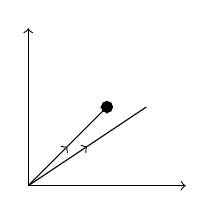
\begin{tikzpicture}
    \draw[->] (0,0) -- (0,2);
    \draw[->] (0,0) -- (2,0);
    \draw[->] (0,0) -- (0.75,0.5);
    \draw[-] (0.75,0.5) -- (1.5,1);
    \draw[->] (0,0) -- (0.5, 0.5);
    \draw[->] (0.5,0.5) -- (1, 1);
    \filldraw (1,1) circle (2pt);
    \end{tikzpicture}
    \caption{Graph 2}
    \label{fig:Gr2}
\end{figure}

As up to translation
\begin{figure}[h!]
    \centering
    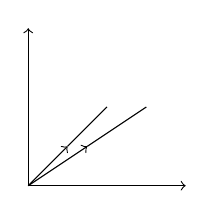
\begin{tikzpicture}
    \draw[->] (0,0) -- (0,2);
    \draw[->] (0,0) -- (2,0);
    \draw[->] (0,0) -- (0.75,0.5);
    \draw[-] (0.75,0.5) -- (1.5,1);
    \draw[->] (0,0) -- (0.5, 0.5);
    \draw[-] (0.5,0.5) -- (1, 1);
    \end{tikzpicture}
    \caption{Graph 3}
    \label{fig:Gr3}
\end{figure}

Vector addition
\begin{figure}[h!]
    \centering
    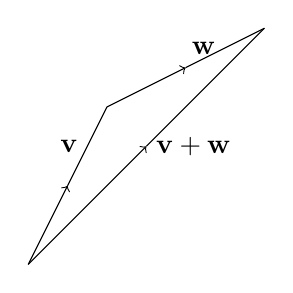
\begin{tikzpicture}
    \draw[->] (0,0) -- (0.5,1);
    \draw[-] (0.5,1) -- (1,2) node [midway, left] {$\mbf{v}$};
    \draw[->] (1,2) -- (2,2.5);
    \draw[-] (2,2.5) -- (3,3) node [midway, left] {$\mbf{w}$};
    \draw[->] (0,0) -- (1.5,1.5) node [right] {$\mbf{v + w}$};
    \draw[-] (1.5,1.5) -- (3,3);
    \end{tikzpicture}
    \caption{Graph 4}
    \label{fig:Gr4}
\end{figure}

Scalar multiplication
\begin{figure}[h!]
    \centering
    \begin{tikzpicture}
    \draw[->] (2,2) -- (3,3) node[left] {$\mbf{v}$};
    \draw[-] (3,3) -- (4,4);
    \draw[->] (2,0) -- (4,2) node[left] {$\mbf{\lambda v}$};
    \draw[->] (4,2) -- (6,4);
    \end{tikzpicture}
    \caption{Graph 5}
    \label{fig:Gr5}
\end{figure}
\textbf{Gr5}


These operations satisfy the \textbf{axioms} of a real vector space.
\begin{enumerate}[label = (\roman*)]
    \item There exists an additive identity $\mbf{0} \in \R ^ n$ such that
    \[
    \mbf{0 + v = v + 0 = v} \ \forall \mbf{v} \in \R ^ n.
    \]
    \item Commutativity
    \[
    \forall\mbf{w, v} \in \R ^ n\quad\mbf{w + v =  v + w}
    \]
    \item Existence of additive inverses
    \[
    \forall\mbf{v} \in \R ^ n\ \exists\mbf{-v} \in \R ^ n \text{ s.t. } \mbf{v + (-v) = (-v) + v = 0}
    \]
    \item Associativity
    $\forall\mbf{u, v, w} \in \R ^ n$
    \[
    (\mbf{u + v}) + \mbf{w} = \mbf{u} + (\mbf{v + w})
    \]
\end{enumerate}
(i), (iii), (iv) $\iff (\R ^ n, +)$ is a group

(i), (ii), (iii), (iv) $\iff (\R ^ n, +)$ is an abelian group \\


\textbf{Axioms} for scalar multiplication
\begin{enumerate}[label = (\roman*)]
    \item $0\mbf{v} = \mbf{0}\quad\forall\mbf{v}\in \R ^ n$.
    \item $1\mbf{v} = \mbf{v}\quad\forall\mbf{v}\in \R ^ n$.
    \item Associativity
    \[
    \lambda (\mu\mbf{v}) = (\lambda\mu)\mbf{v}\quad\forall\lambda,\mu \in \R\quad\forall\mbf{v}\in\R ^ n
    \]
    \item Distributivity, $\forall\lambda,\mu\in\R\quad\forall\mbf{v, w} \in \R ^ n$
    \begin{align*}
    (\lambda + \mu)\mbf{v} &= \lambda\mbf{v} + \mu\mbf{v} \\
    \lambda(\mbf{v + w}) &= \lambda\mbf{v} + \lambda\mbf{w}
    \end{align*}
\end{enumerate}

$\R ^ n$ clearly satisfies these axioms (if not obvious check) because they can be checked component-wise once we set 
\[
-\mbf{v} = \begin{pmatrix}
    -v_1 \\
    -v_2 \\
    \vdots \\
    -v_n
\end{pmatrix}
\]

\begin{definition}
    Standard basis vectors
    
    For $1 \leq i \leq n$ we define $\mbf{e}_i \in \R ^ n$
    \[
    \mbf{e}_i = \begin{pmatrix}
        0 \\
        0 \\
        \vdots \\
        0 \\
        1\footnote{$i$th position from the top.} \\
        0 \\
        \vdots \\
        0
    \end{pmatrix}
    \]    
\end{definition}

\begin{example}
    \[
    \mbf{e}_1 = \begin{pmatrix}
        1 \\
        0 \\
        \vdots \\
        0
    \end{pmatrix}
    \]
    \[
    \mbf{e}_2 = \begin{pmatrix}
        0 \\
        1 \\
        \vdots \\
        0
    \end{pmatrix}
    \]
\end{example}

We can express any vector $\mbf{x} \in \R ^ n$ uniquely as a linear combination of the standard basis vectors.

\begin{example}
    \begin{align*}
    \mbf{x} &= \begin{pmatrix}
        x_1 \\
        x_2 \\
        \vdots \\
        x_n
    \end{pmatrix}
    =
    x_1 \begin{pmatrix}
        1 \\
        0 \\
        \vdots \\
        0
    \end{pmatrix}
    +
    x_2 \begin{pmatrix}
        0 \\
        1 \\
        \vdots \\
        0
    \end{pmatrix}
    +
    \dots
    +
    x_n \begin{pmatrix}
        0 \\
        0 \\
        \vdots \\
        0 \\
        1
    \end{pmatrix} \\
    &= x_1 \mbf{e}_1 + x_2 \mbf{e}_2 + \dots + x_n \mbf{e}_n
    \end{align*}
\end{example}
The $x_i$'s are sometimes called the Cartesian coordinates of the vector $\mbf{x}$.

\subsection{The scalar (or dot) product in $\R ^ n$}

\begin{definition}
    The scalar product is defined as $\R ^ n \times \R ^ n \mapsto \R$, $(\mbf{u, v}) \mapsto \mbf{u \cdot v}$
    \begin{align*}
    \mbf{u \cdot v} &= \begin{pmatrix}
        u_1 \\
        u_2 \\
        \vdots \\
        u_n
    \end{pmatrix} \cdot
    \begin{pmatrix}
        v_1 \\
        v_2 \\
        \vdots \\
        v_n
    \end{pmatrix} \\
    &= u_1 v_1 + u_2 v_2 + \dots + u_n v_n  \\
    &= \sum_{i = 1}^{n}u_iv_i \in \R
    \end{align*}
\end{definition}

\begin{example}
    \[
    \begin{pmatrix}
        4 \\
        1 \\
        2
    \end{pmatrix}
    \cdot
    \begin{pmatrix}
        -3 \\
        -2 \\
        1
    \end{pmatrix}
    =
    -12 - 2 + 2 = -12.
    \]
\end{example}


\textbf{Axioms} of the scalar product
% To-Do add in the foralls here
\begin{enumerate}[label = (\roman*)]
    \item Symmetry
    \[
    \mbf{u \cdot v = v \cdot u}\qquad\forall\mbf{u, v} \in \R ^ n
    \]
    \item Linearity (1)
    \begin{align*}
    (\mbf{u + v)\cdot w}) &= \mbf{u \cdot w + v \cdot w}\qquad\forall \lambda \in \R\\
    \lambda\mbf{u})\cdot \mbf{w} &= \lambda (\mbf{u \cdot w})\qquad\forall\mbf{u, v, w} \in \R ^ n
    \end{align*}
    \item Linearity (2)
    \begin{align*}
        \mbf{u} \cdot (\mbf{v + w}) &= \mbf{u} \cdot \mbf{v} + \mbf{u} \cdot \mbf{w}\qquad \forall \lambda \in \R \\
        \mbf{u} \cdot \lambda\mbf{v} &= \lambda(\mbf{u \cdot v})\qquad \forall\mbf{u, v, w} \in \R ^ n
    \end{align*}
    \item Positivity
    \begin{align*}
        \mbf{v \cdot v} \geq 0\quad \forall \mbf{v} \in \R ^ n \\
        \text{and } \mbf{v \cdot v} = 0 \iff \mbf{v = 0}
    \end{align*}
\end{enumerate}

\begin{definition}
    Given a vector $\mbf{v} \in \R ^ n$ we define its magnitude (or length) to be
    \[
    |\mbf{v}| = \sqrt{\mbf{v \cdot v}}
    \]
\end{definition}
Note $\mbf{v \cdot v} \geq 0$ so positive square roots exist. Likewise note

$|\mbf{v}| \geq 0 \text{ and } |\mbf{v}| = 0 \iff \mbf{v = 0}$

\begin{example}
    \[
    \left|\begin{pmatrix}
        -3 \\
        4
    \end{pmatrix}\right|
    = \sqrt{(-3) ^ 2 + 4 ^ 2} = \sqrt{25} = 5
    \]
\end{example}

Thinking about a vector $\mbf{v} \in \R ^ 2$ where $\mbf{v \neq 0}$
\begin{figure}[h!]
    \centering
    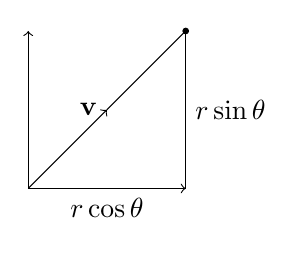
\begin{tikzpicture}
    \draw[->] (0,0) -- (0,2);
    \draw[->] (0,0) -- (2,0);
    \draw[->] (0,0) -- (1,1) node[left] {$\mbf{v}$};
    \draw[-] (1,1) -- (2,2);
    \draw[-] (2,0) -- (2,2) node[midway, right] {$r\sin\theta$};
    \draw[-] (0,0) -- (2,0) node[midway, below] {$r\cos\theta$};
    \filldraw (2,2) circle (1pt);
    \end{tikzpicture}
    \caption{Graph 9}
    \label{fig:Gr9}
\end{figure}

\[
\mbf{v}  = \begin{pmatrix}
    r\cos\theta \\
    r\sin\theta
\end{pmatrix}
\]
where
$r = |\mbf{v}|$ and $0 \leq \theta < 2\pi$, $\theta$ is the angle made by $\mbf{v}$ in an anticlockwise direction with the positive real axis.

We define $(r, \theta) \in (0, \infty) \times [0, 2\pi)$
to be the unique numbers such that
$\mbf{v}  = \begin{pmatrix}
    r\cos\theta \\
    r\sin\theta
\end{pmatrix}$
we call $(r, \theta)$ the polar coordinates of $\mbf{v}$

\begin{example}
    Suppose $\mbf{v} = \begin{pmatrix}
        2 \\
        3
    \end{pmatrix}$,
    what are its polar coordinates?

    $r = |\mbf{v}| = \sqrt{2 ^ 2 + 3 ^ 2} = \sqrt{13}$

    $\theta = \arcsin \left({\dfrac{3}{\sqrt{13}}}\right)$
\end{example}

\begin{example}
    Suppose $\mbf{v} = \begin{pmatrix}
        2 \\
        -2
    \end{pmatrix}$,
    what are its polar coordinates?

    $r = |\mbf{v}| = \sqrt{2 ^ 2 + (-2) ^ 2} = \sqrt{8} = 2\sqrt{2}$

    $\theta = \dfrac{7\pi}{4}$
\end{example}

\begin{proposition}
    Suppose $\mbf{v}, \mbf{w} \in \R ^ n$
    \[
    |\mbf{v}| = r,\quad|\mbf{w}| = s
    \]
    Suppose that $\mbf{v}, \mbf{w}$ make an angle of $\alpha$ with each other $0 \leq \alpha \leq \pi$
    
    Then $\mbf{v}\cdot\mbf{w} = rs\cos(\alpha)$.
    \begin{proof}
        Suppose polar coordinated of $\mbf{v}$ are $(r, \theta)$, and of $\mbf{w}$ are $(s, \varphi)$.

        Then $\mbf{v} = \begin{pmatrix}
            r\cos\theta \\
            r\sin\theta
        \end{pmatrix}$, $\mbf{w} = \begin{pmatrix}
            s\cos\varphi \\
            s\sin\varphi
        \end{pmatrix}$
        \begin{align*}
        \mbf{v\cdot w} &= \begin{pmatrix}
            r\cos\theta \\
            r\sin\theta
        \end{pmatrix} \cdot \begin{pmatrix}
            s\cos\varphi \\
            s\sin\varphi
        \end{pmatrix} \\
        &= rs\cos\theta\cos\varphi + rs\sin\theta\sin\varphi \\
        &= rs(\cos\theta\cos\varphi + \sin\theta\sin\varphi) \\
        &= rs(\cos(\theta - \varphi) \\
        &= rs\cos(\pm\alpha) = rs\cos\alpha.
        \end{align*}
    \end{proof}
\end{proposition}

\begin{corollary}
    If $\mbf{v} \neq \mbf{0}$ and $\mbf{w} \neq \mbf{0}$.
    $\mbf{v}$ and $\mbf{w}$ are orthogonal if and only if
    \[
    \mbf{v \cdot w} = 0.
    \]
    \begin{proof}
        \[
        \mbf{v \cdot w} = 0 \iff \cos(\alpha) = 0 \iff \alpha = \frac{\pi}{2}
        \]
    \end{proof}
\end{corollary}

\begin{example}
    $\mbf{v} = \begin{pmatrix}
        6 \\
        -2
    \end{pmatrix}\qquad
    \mbf{w} = \begin{pmatrix}
        -1 \\
        -3
    \end{pmatrix}$

    Then $\mbf{v\cdot w} = 6(-1) + (-2)(-3) = 0$

    So $\mbf{v, w}$ are orthogonal.
\end{example}


\begin{theorem}[Cauchy-Schwarz inequality]
    Suppose $\mbf{u, v} \in \R ^ n$, $\mbf{u, v} \neq 0$ then we have
    \[
    |\mbf{u}||\mbf{v}| \geq |\mbf{u \cdot v}|
    \]
    with equality if and only if $\mbf{u, v}$ are parallel (multiples of each other).
\end{theorem}

\begin{definition}
    Suppose $\mbf{u, v} \in \R ^ n$ with $\mbf{u, v \neq 0}$ then we define the angle between them to be the unique $0 \leq \theta \leq \pi$ such that $\mbf{u \cdot v} = |\mbf{u}||\mbf{v}|\cos\theta$.
\end{definition}

\begin{example}
    Find the angle between the vectors 
    \[
    \mbf{v} = \begin{pmatrix}
        1 \\ 2 \\ 1 \\ 3
    \end{pmatrix}, \quad \mbf{w} = \begin{pmatrix}
        1 \\ 3 \\ -1 \\ 3
    \end{pmatrix} \in \R ^ 4.
    \]
    Find $\theta$ s.t. $\mbf{v\cdot w} = |\mbf{v}||\mbf{w}|\cos\theta$

    $|\mbf{v}| = \sqrt{1 ^ 2 + 2 ^ 2 + 1 ^ 2 + 3 ^ 2} = \sqrt{1 + 4 + 1 + 9} = \sqrt{15}$
    
    $|\mbf{w}| = \sqrt{1 ^ 2 + 3 ^ 2 + (-1) ^ 2 + 3 ^ 2} = \sqrt{1 + 9 + 1 + 9} = \sqrt{20} = 2\sqrt{5}$

    $\mbf{v \cdot w} = 1 + 6 + -1 + 9 = 15$
    \[
    \cos\theta = \frac{\mbf{v \cdot w}}{|\mbf{v}||\mbf{w}|} = \frac{15}{\sqrt{15}\sqrt{20}} = \frac{\sqrt{15}}{\sqrt{20}} = \frac{\sqrt{3}}{\sqrt{4}} = \frac{\sqrt{3}}{2}
    \]
    $\theta = \dfrac{\pi}{6}$.
\end{example}

For $\mbf{v, w} \in \R ^ n$ $\mbf{v, w \neq 0}$ if $\mbf{v \cdot w} = 0$ (so they make an angle of $\frac{\pi}{2}$) we call $\mbf{v, w}$ orthogonal.

\begin{example}
    Find all unit\footnote{$|\mbf{w}| = 1$} vectors $\mbf{w} \in \R ^ 3$ that make an angle of $\frac{\pi}{4}$ with both.
    \[
    \mbf{u} = \begin{pmatrix} 1 \\ -1 \\ 0 \end{pmatrix},
    \quad\mbf{v} = \begin{pmatrix} 1 \\ 0 \\ 1 \end{pmatrix}.
    \]

    Suppose $\mbf{w} = \begin{pmatrix} w_1 \\ w_2 \\ w_3 \end{pmatrix}$ is a solution.

    First note $|\mbf{u}| = \sqrt{1 ^ 2 + (-1) ^ 2} = \sqrt{2}$,\quad$|\mbf{v}| = \sqrt{1 ^ 2 + 1 ^ 2} = \sqrt{2}$
    Now $\mbf{u \cdot w} = |\mbf{u}||\mbf{w}|\cos\left(\frac{\pi}{4}\right) = \sqrt{2} \cdot 1 \cdot \frac{1}{\sqrt{2}} = 1$

    and $\mbf{v \cdot w} = |\mbf{v}||\mbf{w}|\cos\left(\frac{\pi}{4}\right) = \sqrt{2} \cdot 1 \cdot \frac{1}{\sqrt{2}} = 1$.

    So $w_1 - w_2 = 1$ and $w_1 + w_3 = 1$. So $w_2 = w_1 - 1$ and $w_3 = 1 - w_1$.
    Also $\mbf{w \cdot w} = 1$ so $w_1 ^ 2 + w_2 ^ 2 + w_3 ^ 2 = 1$.
    Hence $w_1 ^ 2 + (w_1 - 1) ^ 2 + (1 - w_1) ^ 2 = 1$
    solve for $w_1$ (two solutions)
\end{example}



\end{document}